%
% Results
\chapter{Results} \label{chap::results}

\section{Simulation Scenario}
To do tests we use a simple scenario. Three static obstacles represent a fence which the system has to overcome. We set the simulation so that the drone has to move back and forth, jumping the fence several times, this is accomplished by switching the start and end points when the distance from the payload to the destination is less than \SI{.3}{\meter}. The simulation runs for \SI{20}{seconds} or until the solver cannot find a solution for 10 consecutive iterations. All the variables of the scenario can be seen in \cref{tab::scenario_data}. An example of a path taken by the system can be seen in \cref{fig::debug_log}.
\begin{table}
	\centering
	\resizebox{\columnwidth}{!}{
	\begin{tabular}{c | l*{14}{c}}
		Variable: & $n$ & $\vec{dim}$ & $\vec p_l$ &$\bar{\vec p}_l$ &  $\vartheta_1$ &  $\varphi_1$ & $\vartheta_2$ &  $\varphi_2$ & $\vec p_{obs_1}$ & $\vec{dim}_{obs_1}$ & $\vec p_{obs_2}$ & $\vec{dim}_{obs_2}$ & $\vec p_{obs_3}$ & $\vec{dim}_{obs_3}$ \\\hline
		\\[-10pt]
		Value: & $2$ & $\begin{bmatrix}
			6\\3\\2.6
		\end{bmatrix}$& $\begin{bmatrix}
		-2.5\\0\\.7
		\end{bmatrix}$& $\begin{bmatrix}
		2.5\\0\\.7
		\end{bmatrix}$
		& 45\degree & 0\degree & -45\degree & 0\degree & $\begin{bmatrix}
		0.01\\-1.2\\0.6
		\end{bmatrix}$ & $\begin{bmatrix}
		0.2\\ 0.2\\ 1.2
		\end{bmatrix}$ & $\begin{bmatrix}
		0.01\\1.2\\0.6
		\end{bmatrix}$ & $\begin{bmatrix}
		0.2\\ 0.2\\ 1.2
		\end{bmatrix}$  & $\begin{bmatrix}
		0.01\\.01\\0.5
		\end{bmatrix}$ & $\begin{bmatrix}
		1\\ 2.4\\ 1
		\end{bmatrix}$ 
		
	\end{tabular}
	}
	\caption{Simulation Scenario Data}
	\label{tab::scenario_data}
\end{table}

\begin{figure}
	\centering
	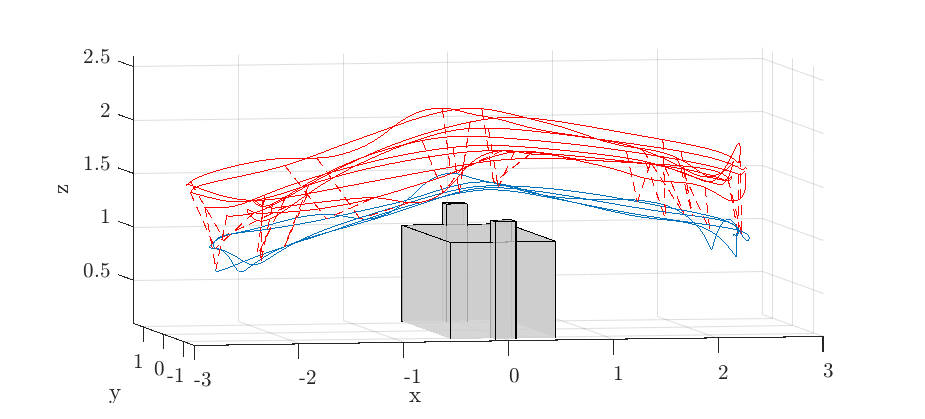
\includegraphics[width=.7\linewidth]{Figures/debug_log}
	\caption{Path of system with $N=20$, $\Delta t=.05$}
	\label{fig::debug_log}
\end{figure}

\section{Estimating time per iteration of the \ac{MPC} solver}
\label{subsect::time_per_it}
In order to set the maximum amount of iterations of the \ac{MPC} solver ($n_{maxit}$), we need to estimate the total time each iteration takes (denoted as \lsymb{$t_{it}$}{Time per iteration}). Even without access to the code from FORCES Pro, it is easy to guess that the time per iteration will depend linearly on the number of stages $N$ but it will not depend on $\Delta t$.

To check this assumption we run the experiments using the initial algorithm (no external planner) with $\Delta t\in\{.1,.05\}$ and $N\in\{10,11,14,17,20,24,29,34,41,50\}$ and on each step of each experiment we record the solve time and the number of iterations required by the solver. Then we plot the time per iteration divided by N using several box-plots. The results of this calculation can be seen in \cref{fig::time_per_it}.

\begin{figure}
	\centering
	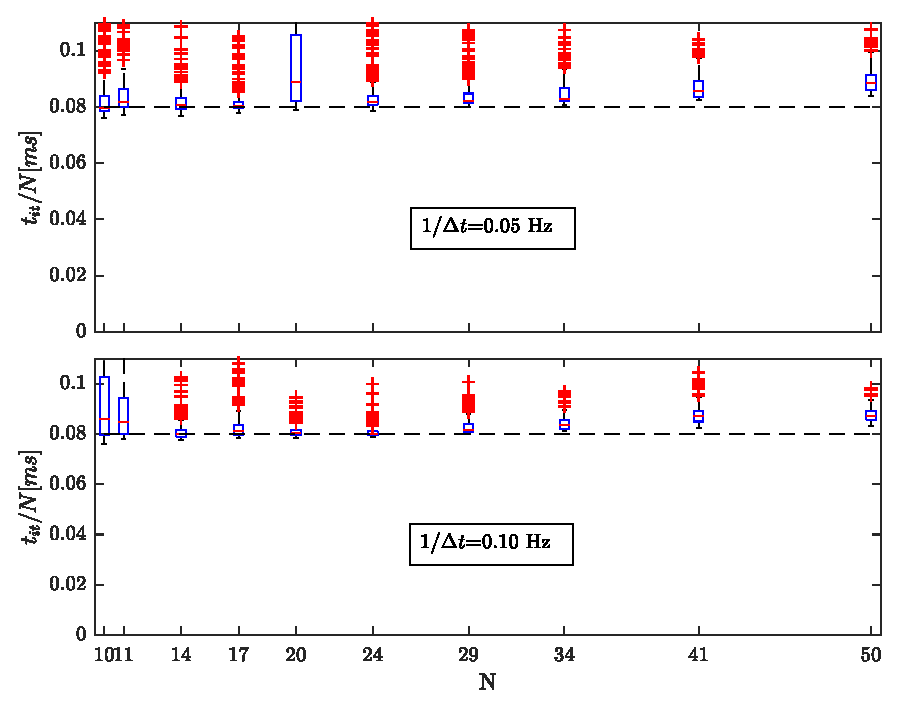
\includegraphics[width=.7\linewidth]{Figures/time_per_it}
	\caption[Graph of $t_{it}/N$]{\nameref{fig::time_per_it} \\ for $\Delta t\in\{.1,.05\}$ and $N\in\{10,11,14,17,20,24,29,34,41,50\}$ \\ A horizontal line is drawn at \SI{.08}{\milli\second}}
	\label{fig::time_per_it}
\end{figure}

Using these results we can see that most iterations run under \SI{.1}{\milli\second} per N, so we can set $n_{maxit}$ using the following equation:
\begin{equation}
\label{eq::maxit}
n_{maxit}=\left\lfloor\frac{\Delta t}{10^{-5}*N}\right\rfloor
\end{equation}

For a different number of drones or obstacles, it is clear that this constant will vary. However, we will not try to model this as the relation is non-linear. Ideally, it would be better to use a solver that can be limited by solve time instead of by the number of iterations. In \cref{fig::time_scaling_quad,fig::time_scaling_obs}, we can see how varying the number of drones or obstacles affects these times. 

\begin{figure}
	\centering
	\begin{minipage}{.5\textwidth}
		\centering
		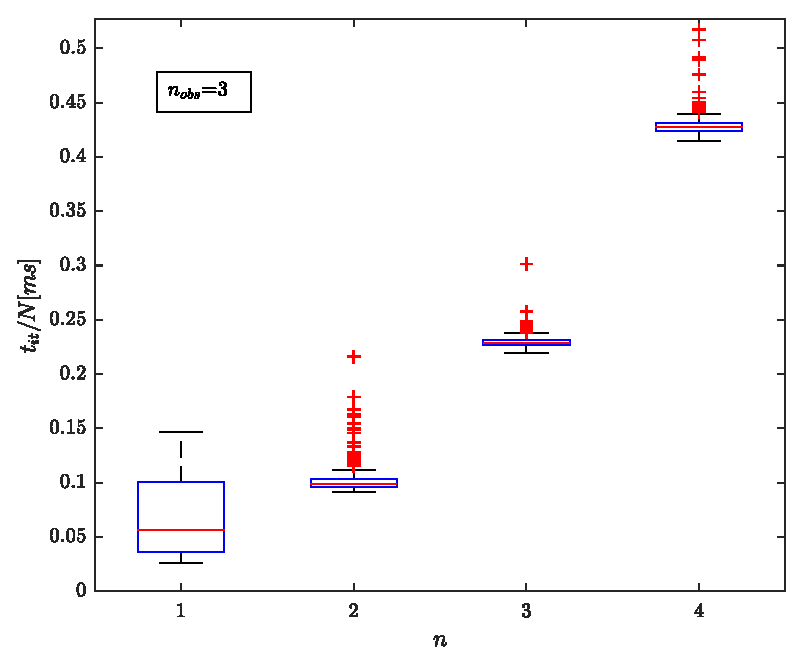
\includegraphics[width=.9\linewidth]{Figures/time_scaling_quad}
		\caption[Scaling of $t_{it}/N$ when varying $n$]{\nameref{fig::time_scaling_quad} with $n_{obs}=3$}
		\label{fig::time_scaling_quad}
	\end{minipage}%
	\begin{minipage}{.5\textwidth}
		\centering
		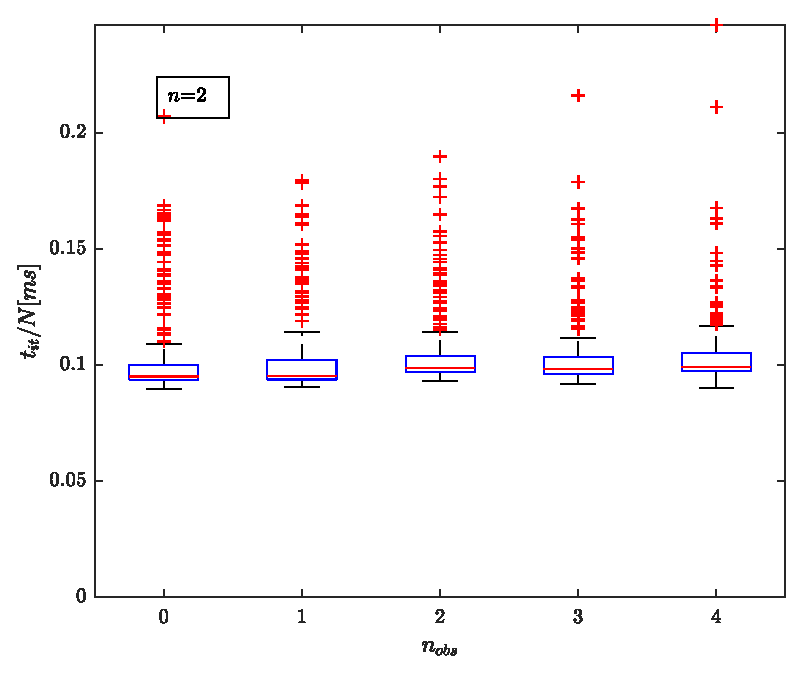
\includegraphics[width=.9\linewidth]{Figures/time_scaling_obs}
		\caption[Scaling of $t_{it}/N$ when varying $n_{obs}$]{\nameref{fig::time_scaling_obs} with $n=2$}
		\label{fig::time_scaling_obs}
	\end{minipage}
\end{figure}


\section{Step time outside the \ac{MPC} solver}
\label{sect::step_time}
When the $\Delta t$ is set to a low amount, the time of the functions other than the \ac{MPC} solver starts to be relevant. We can calculate this time subtracting the \ac{MPC} solve time (\lsymb{$t_{MPC}\in\R_+$}{MPC solve time}) from the time of the control loop (\lsymb{$t_{step}\in\R_+$}{Control loop time}) We calculated these times using the same parameters as the ones used in \cref{subsect::time_per_it}.

As it can be seen in \cref{fig::time_per_step}, these results do not seem to follow a pattern that is easy to model, so we will not try to model this and will assume that they are zero, this however will make the loop time slower than intended when setting $\Delta t$ to a small value.

\begin{figure}
	\centering
	\begin{center}
		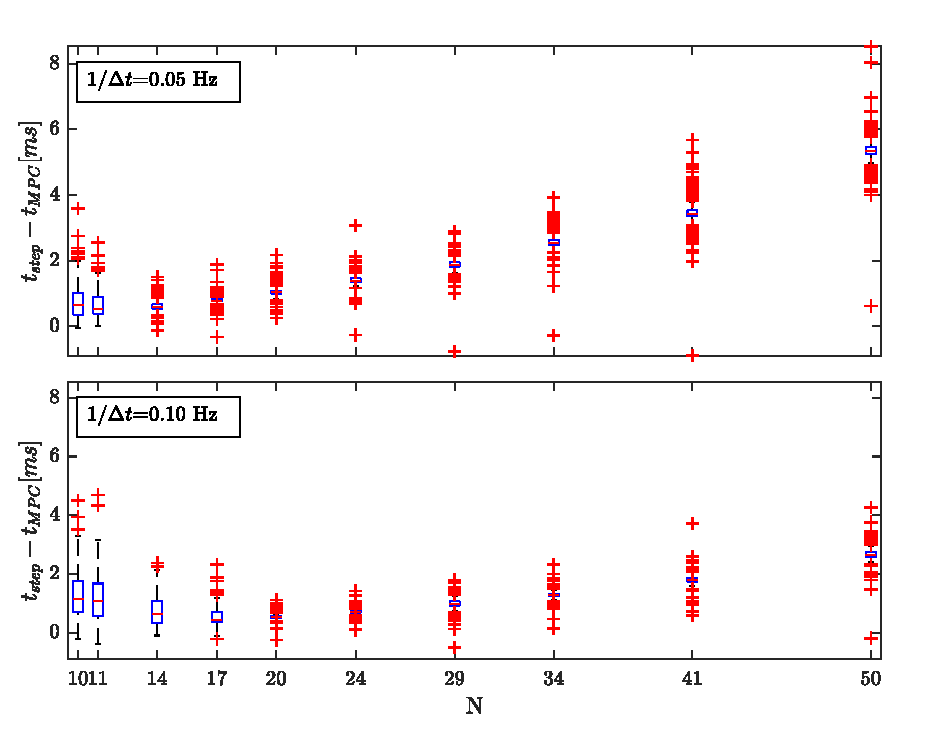
\includegraphics[width=.7\linewidth]{Figures/time_per_step}
	\caption[Graph of $t_{step}-t_{MPC}$]{\nameref{fig::time_per_step} \\ for $\Delta t\in\{.1,.05\}$ and $N\in\{10,11,14,17,20,24,29,34,41,50\}$}
	\label{fig::time_per_step}
	\end{center}
\end{figure}

\section{Finding best parameters}
We then ran some more tests to find the best parameters. We tested the same problem as in the previous sections with different $\Delta t$ and different time horizons (defined by $t_{horizon}=N\Delta t$ \hiddenlsymb{$t_{horizon}\in\R_+$}{Planning time horizon}). For each time horizon $N$ is found using the formula $N=\left\lceil\frac{t_{horizon}}{\Delta t}\right\rceil$. The results of these experiments are seen in \cref{fig::time_horizon}.

\Needspace{10\baselineskip}
From these results, and from further inspections on the data we concluded the following:
\begin{itemize}
	\item If the time horizon is too low, the system will break constraints more often. This makes sense as with a low time horizon the drone does not have time to react to the obstacles. As a good rule of thumb, the time horizon should be greater than the time needed for the system to stop.
	\item If the time horizon is too high the $N$ is high and following \cref{eq::maxit},$n_{maxit}$ will be smaller. Therefore, the quality of the results decrease (this cannot be seen in \cref{fig::time_horizon} but on inspection of the data obtained). 
	\item When the $\Delta_t$ is too high ($1/\Delta_t$ too low), the system tends to have more problems. This is mainly due to the errors that come from a rough discretization of the dynamics.
	\item When the $\Delta_t$ is too low ($1/\Delta_t$ too high), as explained on \cref{sect::step_time}, the loop time outside the \ac{MPC} solver will not be negligible and the loop will run slower than intended.
\end{itemize}

Taking into account all of this information, it was decided to have a time horizon of \SI{1.2}{\second} and a $\Delta t$ of \SI{0.083}{\second} (\SI{12}{\hertz}). Therefore the $N$ will have a value of $15$.

\begin{figure}
	\centering
	\begin{center}
		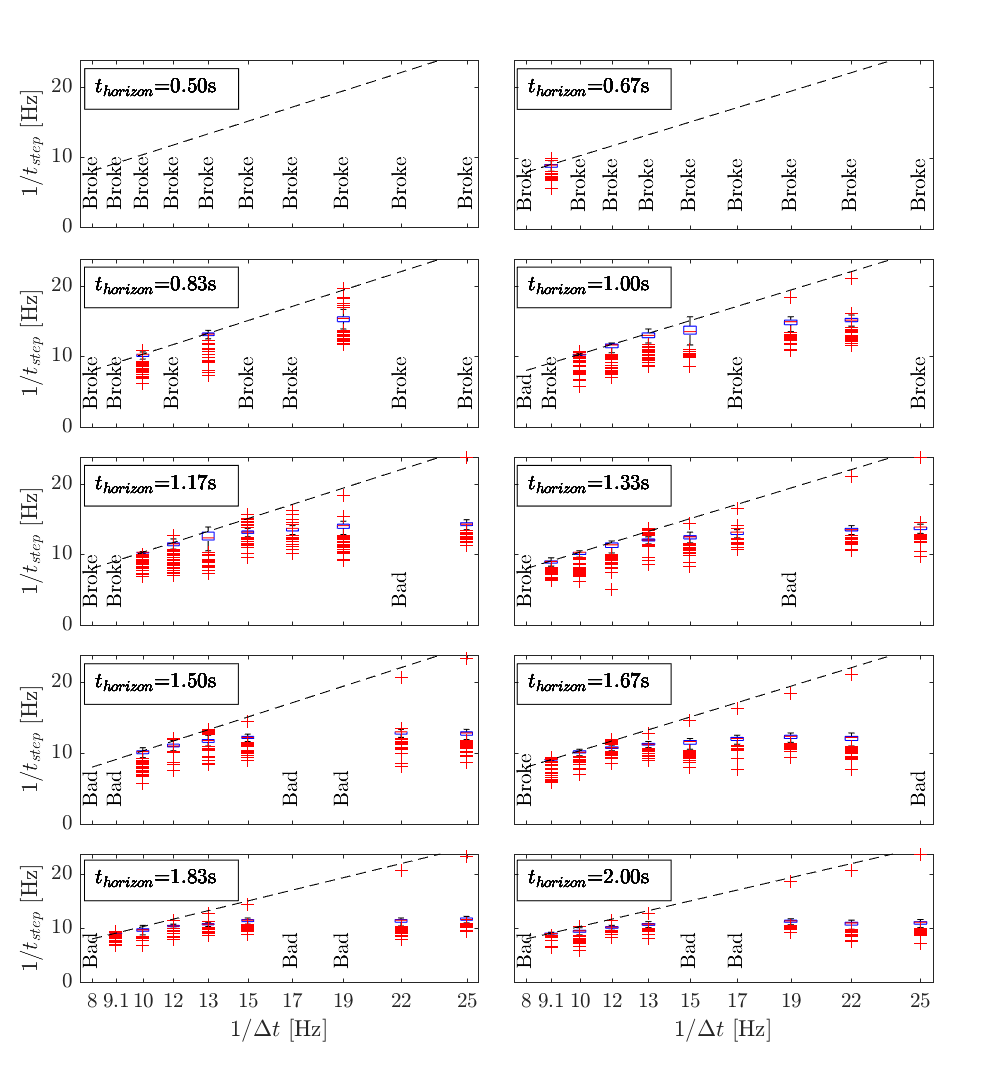
\includegraphics[width=1\linewidth]{Figures/time_horizon}
		\caption[Graph of $1/t_{step}$]{\nameref{fig::time_horizon} for $1/\Delta t\in\{8.0, 9.08, 10.3, 11.7, 13.3, 15.1, 17.1, 19.4, 22.0, 25.0\} \si{\hertz}$ and $t_{horizon}\in\{\frac{1}{2} , \frac{2}{3} , \frac{5}{6} , 1 , \frac{7}{6} , \frac{4}{3} , \frac{3}{2} , \frac{5}{3} , \frac{11}{6} , 2 \} \si{\second}$ \\ When the system broke any constraint for more than 1\% of the time it is marked as "Broke" \\When the system did not manage to cross the fence more than 3 times it is marked as "Bad" \\ A line marks the $t_{step}<\Delta t$ maximum.}
		\label{fig::time_horizon}
	\end{center}
\end{figure}

\section{External planner testing}
When we are using an external planner, we can no longer use the assumption that the drone has followed exactly the \ac{MPC} plan. Therefore we need to find the initial solution for the \ac{MPC} solver using the algorithm described in \cref{subsect::initial_solution}.

When testing the external planner algorithm we set the maximum number of iterations to a factor of the previous calculation. This factor, \lsymb{$k\in\R_+$}{Maximum iteration factor for external planner}, sets the maximum amount of stages the controller could perform without a new plan. 

\begin{equation}
\label{eq::maxit_k}
n_{maxit}=\left\lfloor\frac{k\Delta t}{10^{-5}*N}\right\rfloor
\end{equation}

As it was explained before, this algorithm was not successful, as it performed worse than the original algorithm. This was true for several values of k tested. The possible causes are:
\begin{itemize}
	\item The initial solution is poor, this means the solver takes more time to find the optimal solution and therefore, the next plan will have an even worse initial solution.
	\item The algorithm to determine the best inputs depending on the location of the drone does not perform well when the drone is far away from the plan.
	\item Even when the drone is in the path of the plan, it can be in between two of the planned stages, this causes the drone to follow inputs that were meant to be executed at a slightly different time.
\end{itemize}

\section{Demonstration of Maneuvers}
We will now demonstrate some maneuvers that our system is able to calculate. A video of these maneuvers can be seen in \url{https://youtu.be/lECcAQC_coE}.

\subsection{Moving obstacle avoidance}
To demonstrate moving obstacle avoidance a scenario is designed where two drones move from side to side while some obstacles move perpendicularly through the optimal path. 

In order to make it easier to visualize the movement from a top-down view, the obstacles are set to have a very large height, much larger than the workspace dimensions.

In \cref{fig::zigzag} we can see one of these maneuvers:

In (\ref{subfig::zigzag::start}) we see how the system is dodging obstacle 2. However, it is not doing anything to prevent a collision with obstacle 1, as it is not yet within the time horizon of the controller. 

In (\ref{subfig::zigzag::stop}) we see how obstacle 1 is now on the system's time horizon. Quadrotor 4 has already found a way to avoid the obstacle while quadrotor 3 is trapped, it cannot go forward as it assumes that the obstacle will be there in the future and it cannot turn to the right as it would crash against quadrotor 4, therefore the quadrotor 3 plans to stop as closely as possible to its objective. Also, note how quadrotor 3 stops in a way that makes the payload swing backward, avoiding a collision between the payload and the obstacle.

In (\ref{subfig::zigzag::found}) quadrotor 4 has followed its plan and is moving forward. This has given quadrotor 3 enough space to move behind quadrotor 4 and move towards its objective. Note how at the end of the planned path of quadrotor 3, it is not dodging the current position of the obstacle but its expected position.

Finally, in (\ref{subfig::zigzag::end}) we see how the system has successfully avoided the obstacle and is moving towards the objective.

\begin{figure}
	\centering
	\begin{subfigure}{0.45\textwidth}
		\centering
		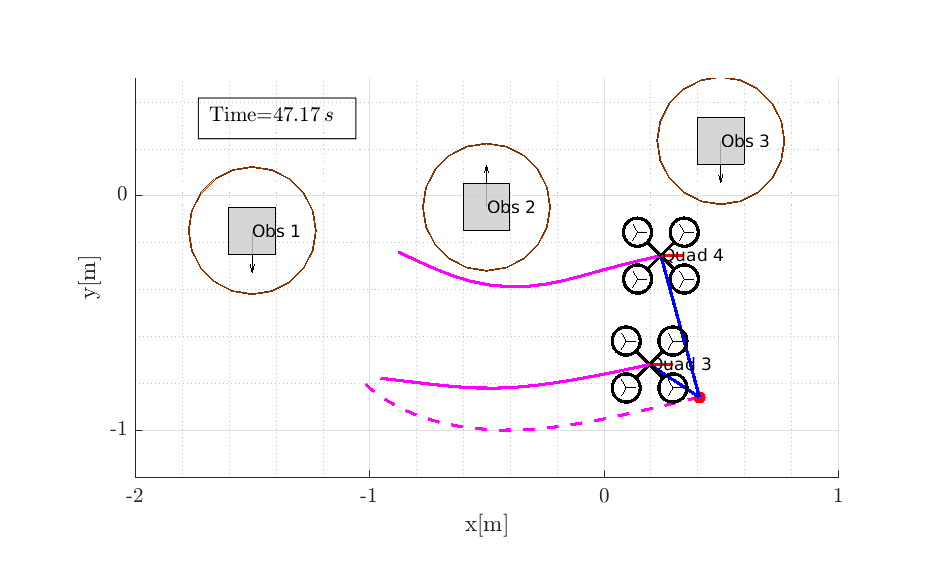
\includegraphics[width=\textwidth]{Figures/zigzag/start}
		\caption{Starting position of maneuver}
		\label{subfig::zigzag::start}
	\end{subfigure}
	\begin{subfigure}{0.45\textwidth}
		\centering
		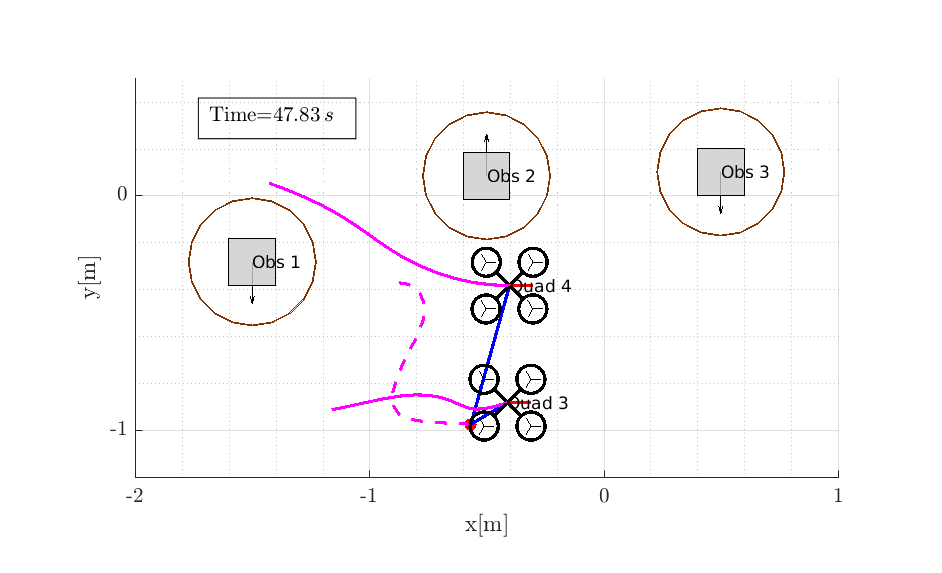
\includegraphics[width=\textwidth]{Figures/zigzag/stop}
		\caption{One drone stops}
		\label{subfig::zigzag::stop}
	\end{subfigure}
	\begin{subfigure}{0.45\textwidth}
		\centering
		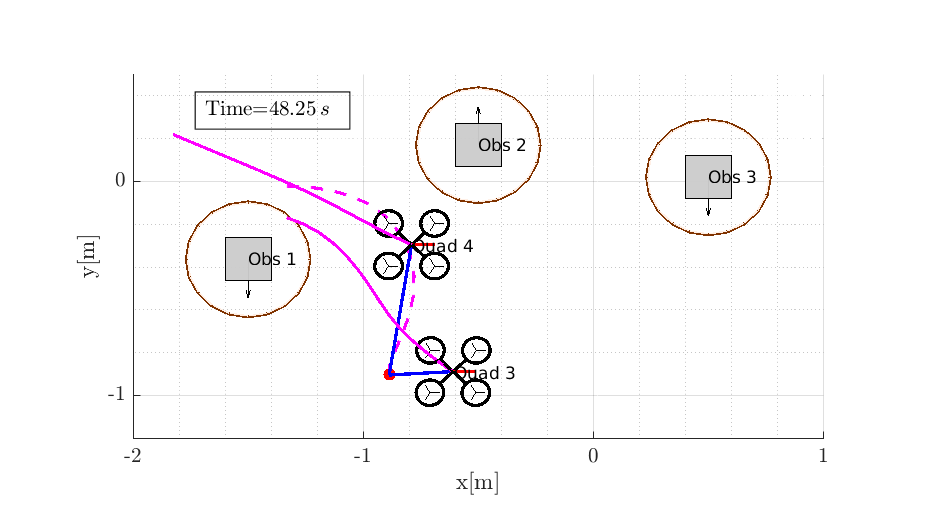
\includegraphics[width=\textwidth]{Figures/zigzag/found}
		\caption{A solution is found}
		\label{subfig::zigzag::found}
	\end{subfigure}
	\begin{subfigure}{0.45\textwidth}
		\centering
		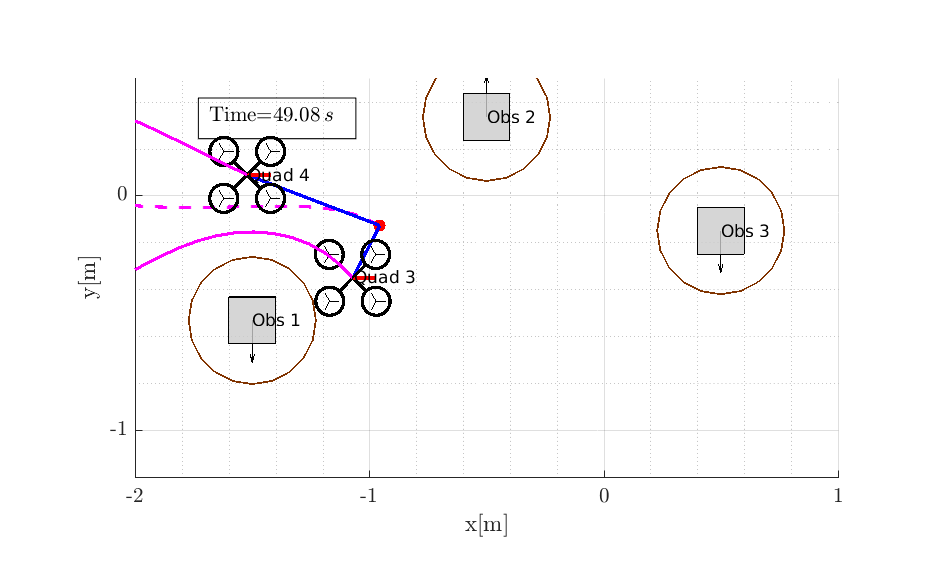
\includegraphics[width=\textwidth]{Figures/zigzag/end}
		\caption{The system avoids the obstacle}
		\label{subfig::zigzag::end}
	\end{subfigure}
	\caption[Moving obstacle avoidance]{\nameref{fig::zigzag}\\Plotted with the same rules as the ones explained in \cref{sect::visualizer} (\nameref{sect::visualizer})\\Black lines have been added to represent the obstacles' velocities\\For each instance, the top view is shown}
	\label{fig::zigzag}
\end{figure}

\subsection{High swing maneuvers}
In order to demonstrate maneuvers that utilize swing, we create a new scenario where two drones have to overcome a horizontal barrier that is in the way. To prevent the drones from simply going over it, we change the workspace limits to set a ceiling at a height of \SI{1}{\meter}. In order to exaggerate the movement, we increase the limit set to the swing angles in \cref{eq::linear_ineq} from \SI{60}{\degree} to \SI{85}{\degree}. 

In \cref{fig::highpole} we can see one of these maneuvers:


\begin{figure}
	\centering
	\begin{subfigure}{0.9\textwidth}
		\centering
		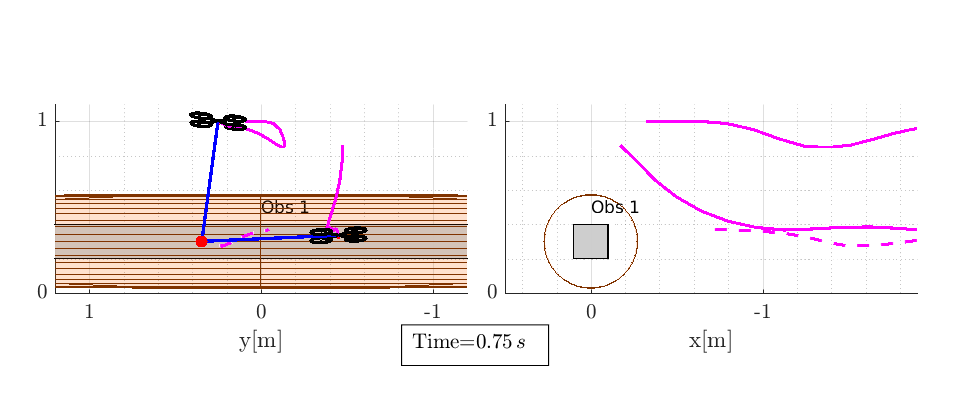
\includegraphics[width=\textwidth,trim={0 0 0 1cm},clip]{Figures/highpole/stop}
		\caption{The system does not yet know how to pass the obstacle}
		\label{subfig::highpole::stop}
	\end{subfigure}
	\begin{subfigure}{0.9\textwidth}
		\centering
		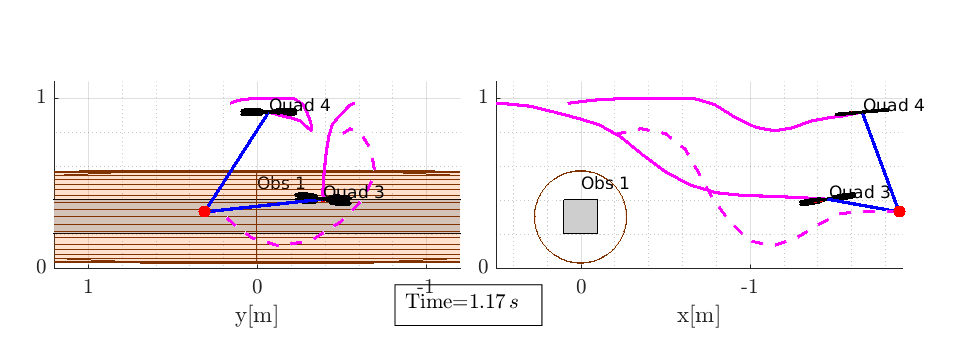
\includegraphics[width=\textwidth,trim={0 0 0 1cm},clip]{Figures/highpole/found}
		\caption{The system seems to have found a solution}
		\label{subfig::highpole::found}
	\end{subfigure}
	\begin{subfigure}{0.9\textwidth}
		\centering
		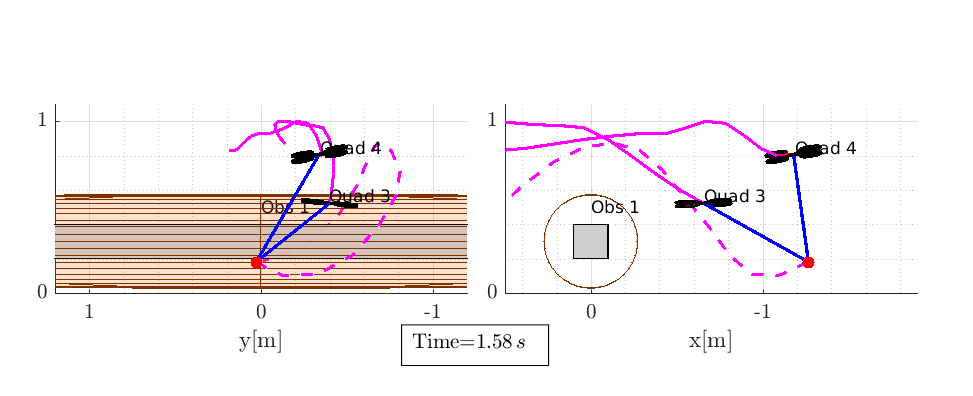
\includegraphics[width=\textwidth,trim={0 0 0 1cm},clip]{Figures/highpole/moving}
		\caption{The system moves closer}
		\label{subfig::highpole::moving}
	\end{subfigure}
	\begin{subfigure}{0.9\textwidth}
		\centering
		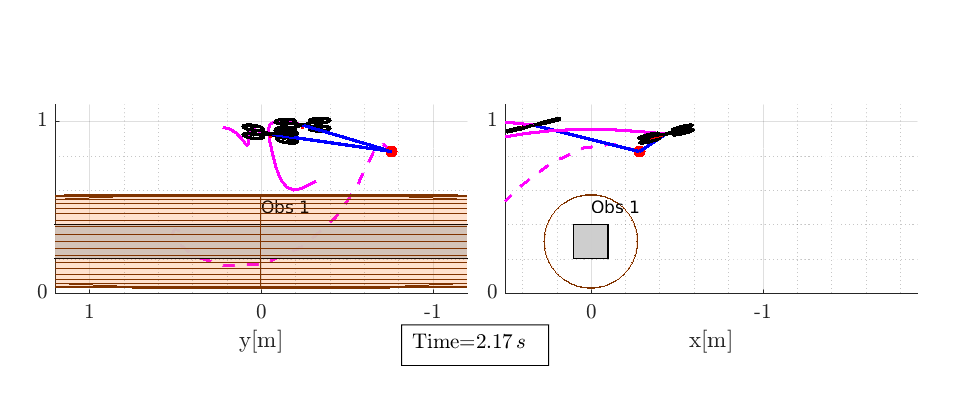
\includegraphics[width=\textwidth,trim={0 0 0 1cm},clip]{Figures/highpole/swing}
		\caption{The system swings the payload over the obstacle}
		\label{subfig::highpole::swing}
	\end{subfigure}
	\caption[High swing maneuver]{
		\nameref{fig::highpole}\\Plotted with the same rules as the ones explained in \cref{sect::visualizer} (\nameref{sect::visualizer}) \\ For each instance, two side views are shown}
	\label{fig::highpole}
	
\end{figure} 

In (\ref{subfig::highpole::stop}) the drones have just encountered the obstacle within the system's time horizon and have not yet found a solution to go over it, therefore the drones plan to get  as close as they can to the objective while staying behind the obstacle.

In (\ref{subfig::highpole::found}) the system seems to have found a solution to overcome the obstacle and the drones are starting to execute it.

In (\ref{subfig::highpole::moving}) the system has moved closer to the obstacle, and we can more clearly see what the plan was. Both drones have positioned themselves perpendicularly to the obstacle and are planning to swing the payload to the side while they go above the obstacle. This highly complex maneuver is only possible thanks to having a high time horizon and a good definition of the cost function.

In (\ref{subfig::highpole::swing}) we see how the payload is swinging above the obstacle and how each of the drone starts planning a path to move to their respective objectives.

\section{Experimental Results}
\label{sect::experimental}

Due to time limitations, very few experiments were performed with real drones and on none of them we got good enough results. 

Observing the logs of data obtained from these failures it was found that the system was generating correct \ac{MPC} plans and the system seemed to follow them correctly, which is promising. However, the length of the cables did not match the real distance between the payload and the quadrotors and, as in our model the position of the drones is determined by the position of the payload and the suspension angles (\cref{eq::pi}), this causes the position of the drones to be different in the model than in reality and the system destabilizes.

A boxplot of the real distances can be seen in \cref{fig::real_len}, we can see how these distances vary considerably. This is because the cables are not attached to the center of mass of the drones but to a different point. 

\begin{figure}
	\centering
	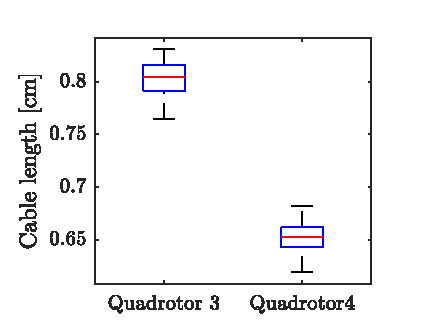
\includegraphics[width=.3\linewidth]{Figures/real_len}
	\caption{Real distance between the payload and the quadrotors} 
	\label{fig::real_len}
\end{figure}

With more time to experiment it could be possible to attach the drones differently or control the payload using longer cables so that this difference is minimized. Another solution would be to set the length of the cables as a parameter of the \ac{MPC} solver and set it to the real distance of the drones. It would also be a possibility to change the dynamic model to account for the difference the swing point of the cables and the center of mass of the quadrotors. A higher control rate would also help stabilize the system.

